\section{Protocolo NTP}
\label{sec:NTP}

O Network Time Protocol é um protocolo de sincronização de relógios que sincroniza os relógios de um sistema distribuído através de redes com comutação de pacotes e de latência variável, com uma precisão na ordem dos milissegundos. Este protocolo foi, primordialmente, concebido para ter uma alta exatidão e fiabilidade \cite{b2}.

Para uma típica operação do NTP, o cliente questiona um ou mais servidores NTP e recebe o tempo atualizado segundo o servidor. Após a receção dos dados do servidor, o cliente calcula o offset e o rate do seu relógio relativamente ao servidor e o delay da rede. Para tal, é necessário que ele saiba os timestamps da mensagem enviada por ele ao servidor e da consequente resposta. A figura \ref{fig:diagramaNTP} ilustra uma execução do protocolo. Os timestamps necessários para o cálculo dos parâmetros de sincronização são: tempo em que pedido é enviado pelo cliente, t0, tempo em que o pedido é recebido pelo servidor, t1, tempo em que a resposta é enviada pelo servidor, t2 e tempo em a resposta é é recebida pelo cliente, t3.

    \begin{figure}[h]
        \centering
        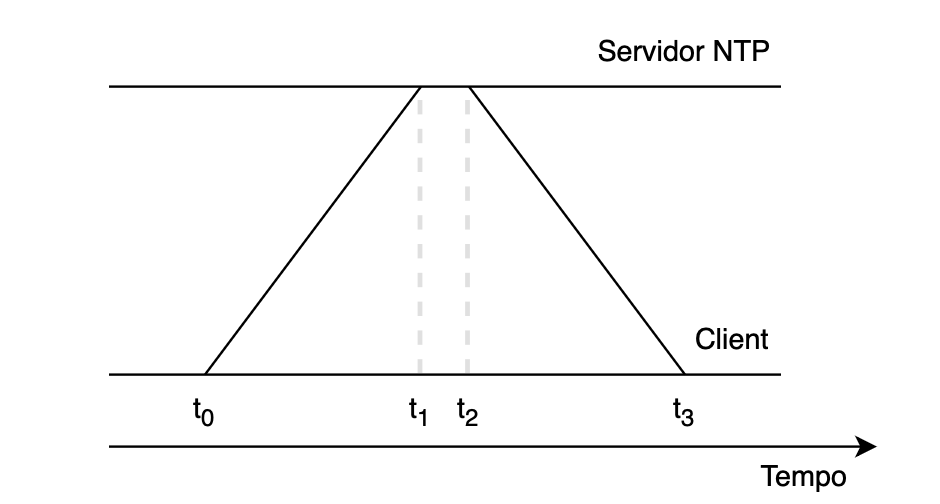
\includegraphics[width=0.8\linewidth]{figures/diagramaNTP.png}
        \caption{Ordem de eventos do protocolo NTP}
        \label{fig:diagramaNTP}
    \end{figure}

Com estes 4 tempos é possível inferir os seguinte parâmetros:
\begin{outline}
    \1 Offset, $\theta$:  corresponde à diferença entre o relógio do cliente e do servidor, equação\ref{eq:offset}.
    \1 Delay, $\delta$: corresponde ao tempo que o pedido demora a chegar ao servidor, equação \ref{eq:delay}.
    \1 Rate, $\rho$: razão entre a velocidade de incrementação do relógio do servidor e do cliente, equação \ref{eq:rate_sem_delay}
\end{outline}


\begin{subequations}
    \begin{equation} \label{eq:offset}
    \theta = \frac{\left( (t_{\text{1}} - t_{\text{0}}) + (t_{\text{2}} - t_{\text{3}}) \right)}{2} 
    \end{equation}
    
    \begin{equation} \label{eq:delay}
    \delta = (t_{\text{3}} - t_{\text{0}}) - (t_{\text{2}} - t_{\text{1}})
    \end{equation}
    
    \begin{equation} \label{eq:rate_sem_delay}
    \text{{rate}} =\left| \frac{{t_{\text{1}}' - t_{\text{1}}}}{{t_{\text{0}}' - t_{\text{0}}}} \right|
    \end{equation}
    \label{eq:parametros}
\end{subequations}

Na equação \ref{eq:rate_sem_delay}, os valores $t_{\text{0}}'$ e $t_{\text{1}}'$ correspondem aos timestamps mais recentes, enquanto t1 e t0 correspondem aos timestamps da sincronização anterior. Deste modo, o rate apenas depende das duas últimas iterações entre cliente-servidor. Contudo, esta equação não tem em conta o delay da rede, sendo que este nunca é constante e influencia o valor do rate. Na figura \ref{fig:diagramaNTP_delays} observa-se o efeito do delay da rede para o período NTP, ou seja o período entre $t_1$ e $t_1'$ ($T_{NTP} = t_1'-t_1$). Idealmente, o delay é constante com o valor $\mu$. Contudo, no caso em que um pedido sofra um delay menor que o esperado, $d$, e o seguinte um delay maior que o esperado, $d'$, o valor de $T_{NTP}$ será superior ao real, de acordo com a equação \ref{eq:pior_caso}, levando a que o cliente julgue que precise uma variação de rate superior à real. 


\begin{figure}[h]
        \centering
        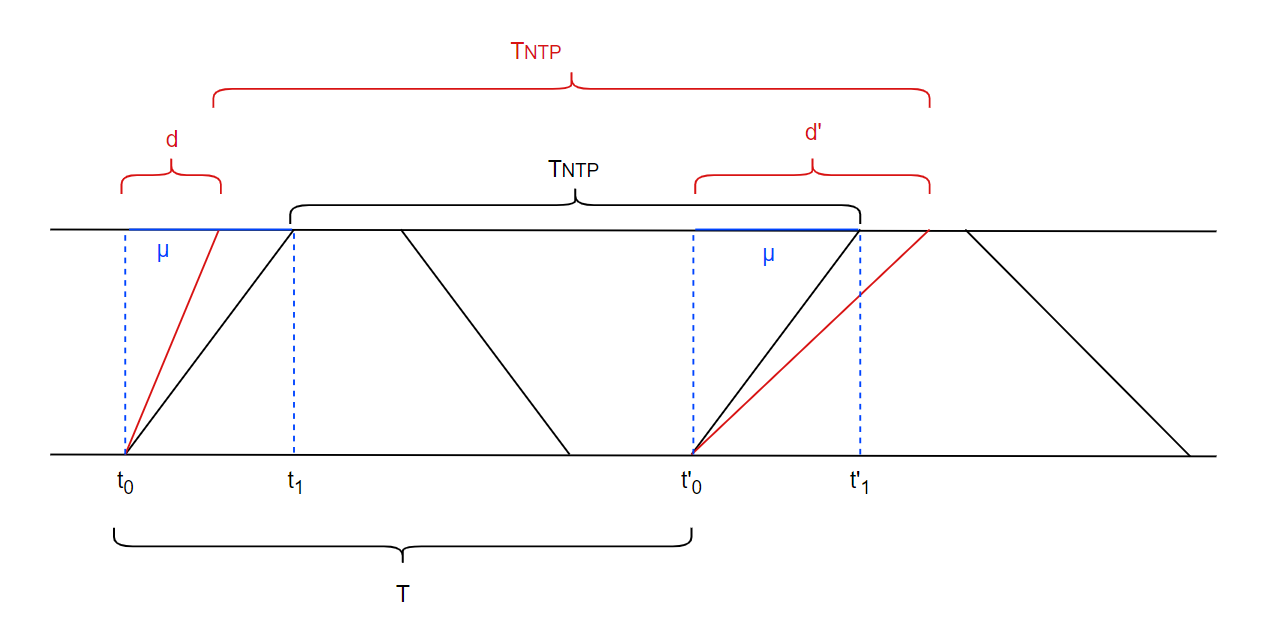
\includegraphics[width=1.0\linewidth]{figures/diagrama_ntp_delay.png}
        \caption{Efeito da variação do delay no período NTP}
        \label{fig:diagramaNTP_delays}
\end{figure}

\begin{equation} \label{eq:pior_caso}
    T_{NTP_{incorreto}} = T_{NTP} + d + d'
\end{equation}

Deste modo, para contrariar este tipo de casos, o valor esperado do delay é atualizado a cada sincronização de acordo com a equação \ref{eq:media_delay}. A cada sincronização, é calculado o erro introduzido pela variação do delay (equação \ref{eq:delay_medio}) e descontado no cálculo do rate, equação \ref{eq:rate_com_delay}.


\begin{subequations}
    \begin{equation} \label{eq:media_delay}
        \mu_k = \frac{N \times \mu_{k-1} + \delta_k}{N+1}
    \end{equation}
    
    \begin{equation} \label{eq:delay_medio}
        \varepsilon = \mu - \delta + \mu - \delta'
    \end{equation}
    
    \begin{equation} \label{eq:rate_com_delay}
        \rho = \left| \frac{t'_1 - t_1 -\varepsilon}{t'_0-t_0} \right|
    \end{equation}
\end{subequations}



Por fim, sempre que o cliente precisar de utilizar um tempo sincronizado, irá calcular o tempo que passou desde a última atualização de acordo com o seu relógio (não sincronizado), multiplicado pelo rate, somado com o offset e adicionado ao tempo da última sincronização. 

\begin{equation} \label{eq:corrected_time}
    \text{{corrected\_time}} = t_{\text{0}}' + \text{{elapsed\_time}} \cdot \text{{rate}} + \theta
\end{equation}



